
\chapter{Introduction}
% 학위논문 주제 설정의 배경, 관련 분야에서 기존의 연구,
% 본 논문의 취지, 실험 논문의 경우 연구에 대한 간략한 소개와
% 연구를 위해 설정한 가설 등을 소개한다.
\section{Sequence Databases}

Next generation sequencing (NGS) technologies have revolutionized the way we collect and analyze biological data.
Thanks to NGS, the cost of sequencing has dropped drastically and continued to decrease with more new technologies developed.
Accompanying this change is the explosive growth of the amount of sequencing data and the size of sequence databases.
The Sequence Read Archive (SRA) is one of the most popular and widely used sequence databases that store both private and public sequence reads and provide access in various foramts including the commonly used \texttt{FASTQ} file format.
Its size has grown exponentially since 2008 and currently reached more than 60 petabytes large.
The growth in size of Sequence Read Archive is visualized in \autoref{fig:sra_stat}.
Among all 16,700,872 SRA samples shown in SRA sequence browser, merely searching with they keyword "metagenome" already gives 2,176,719 results.
Such a huge amount of metagenomic data is a valuable resource for many research projects including drug discovery, environment conservation, and finding candidates for bioengineering.

\section{State-of-the-art Algorithms for Sequence Searches}

Due to the extensive size of the Sequence Read Archive and other sequence databases, it is a challenge to provide much needed algorithms to search against the vast amount of data.
The classical \texttt{BLAST} and \texttt{BLASTX} are sensitive but slow \cite{altschul1990basic}, thus not feasible for an all-encompassing search through petabyte-scale databases or other high-throughput scenarios.
Although there were attempts to use cloud computing to speed up the search process \cite{levi2018searching}, the base performance of the algorithms were not improved.
Algorithms such as \texttt{MMseqs2} \cite{steinegger2017mmseqs2}, \texttt{DIAMOND} \cite{buchfink2015fast} and \texttt{BIGSI} \cite{bradley2019ultrafast} are some of the most promising ones that strike a good balance between sensitivity and speed.
However, they are still not capable of handling terabyte-scale data.

\section{Motivation and Contribution of the Thesis}

In conclusion, the search of homologs in large sequence databases requires a fast yet sensitive enough algorithm specially designed for petabyte-scale analysis.
The state-of-the-art searching algorithms failed to satisfy this need.
To tackle these problems and, we developed the \texttt{Petasearch}.
Jonas H{$\ddot{u}$}gel first proposed and impelmented the prototype of \texttt{Petasearch} in his Master's thesis in collaboration with Milot Mirdita.
The thesis author revised the design of the core data structures and database format of \texttt{Petasearch}, integrated new modules, and added the profile-search functionality, pushing the algorithm to a finishing state.
The thesis author also impelmented new benchmarks, prepared metagnomic assembly for \texttt{Petasearch} to search on, and conducted two explorative analyses using \texttt{Petasearch}.
The main contribution of this thesis is the major improvement of the \texttt{Petasearch} algorithm in speed, space consumption and sensitivity.

In \cref{chapter:materials-methods}, we will start with introducing the current overview of the \texttt{Petasearch} algorithm, and continue with describing the its further development and optimization.
We will also describe the design of the benchmarks in \cref{chapter:materials-methods}.
In \cref{chapter:results}, we will first show the improvements in efficiency and effectiveness of the forementioned optimizations.
Afterwards, we will show a thorough comparison of the performance of the \texttt{Petasearch} algorithm with the state-of-the-art algorithms.
In \cref{chapter:discussion}, we will discuss the potential application of \texttt{Petasearch} and show two examples of its usage.

% \pagebreak

% \begin{figpage}
\begin{figure}[htbp]
  \centering
  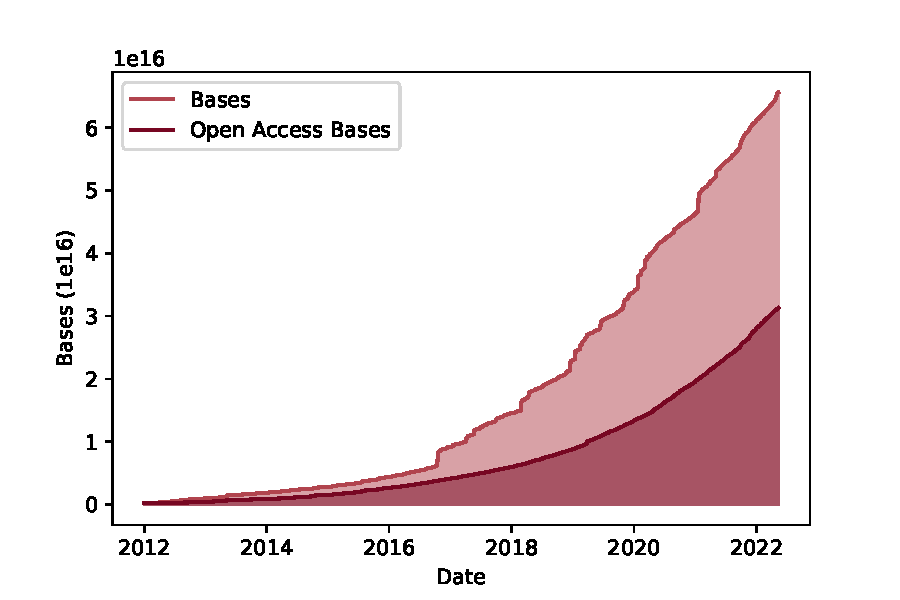
\includegraphics[width=\textwidth]{images/sra_stat.pdf}
  \caption{\textbf{The exponential growth of the Sequence Read Archive over the decade (from 2012 to 2022).}
The total amount of sequence data (unit in bases) and publicly available data are visualized in pink and dark red respectively.}
  \label{fig:sra_stat}
\end{figure}
\pagebreak
% \begin{figure}
  % \includegraphics[]{}
% \end{figure}
% \end{figpage}
